% !TEX root = ../../../main/aws_chabauty.tex
\newpage
\section{Bjorn Poonen: Introduction to Chabauty's method and Kim's nonabelian generalization}
\subsection{Lecture 1}
\subsubsection{Rational points on Curves}

The starting point is Falting's Theorem, which was originally known as Mordell's conjecture.

\begin{thm}[Falting's, 1983]
Suppose $[K \colon \Q] < \infty$, and let $X$ be a `nice'\footnote{smooth, projective, geometrically integral} curve of genus $g$ over $K$. If $g>1$, then $X(K)$ is finite. 
\end{thm}


There are several proofs now. The first was Falting's proof in 1983 based on Arakelov methods. The next was by Vojta 1991 and its variant (phrased in more elementary terms via Diophantine approximation) by Bomberi. But now there is a proof by Lawrence-Venkatesh in 2018 via $p$-adic period maps. 


For integral points, the parallel to Falting's Theorem is Siegel's Theorem. Let $[K \colon \Q] < \infty$. Let $\O= \O_{K,S}= \{ x \in K \colon \nu(x) \geq 0 \text{ for all } \nu \in S \}$, where $S$ is a finite set of places, including all the archimedean places. Let $U:= X \setminus Z$, where $X$ is a nice curve of genus $g$ and $Z$ is a nonempty 0-dimensional subscheme. Now $\chi(U):= (2-2g) - r$, where $r= \#Z(\overline{K})$ and $\chi(U)$ is the topological Euler characteristic of $U$. Of course, $U$ is a scheme over $K$, so strictly speaking it does not make sense to speak of integral points. In order to talk about integral points, we need to choose a model for $U$ over $\O$, we call this $\cU$. So suppose $\cU$ is a finite type $\O$-scheme with $\cU_K\simeq U$. If $\chi(U)< 0$, then $\cU(\O)$ is finite. The condition that $\chi(U)<0$ is sometimes phrased as `$U$ is hyperbolic' [over $\C$, $\widetilde{U} \simeq b$]. 


\begin{thm}[Siegel's Theorem, 1929]
If $\chi(U)< 0$, then $\cU(\O)$ is finite. 
\end{thm}


There is a proof, obviously, by Siegel. But there are also proofs by Baker-Coates (1970) when either $g \leq 1$ or when $U$ is $y^2= f(x)$ in $\A^2$, and Lawrence-Venkatesh (2018) when $U= \P^1 \setminus \{0,1,\infty\}$. 


\begin{ex}
If $U= \P \setminus \{0,1,\infty\}$ and $\cU= \spec \O[x, \frac{1}{x},\frac{1}{1-x}]$. Then $\cU(\O)$ is the set of solutions to $x+y=1$ with $x,y \in \O^\times$. 
\end{ex}


\begin{rem}
Falting's Theorem is strictly harder than Siegel's Theorem in that Falting's Theorem implies Siegel's Theorem. The key idea is that if $\chi(U)<0$, then there is some finite \etale cover of the affine curve $U$ that is open in a `nice' curve of genus greater than 1. Using descent theory, you can reduce the problem of finding integral points on $U$ to finding integral points on the cover (and perhaps some of its twists). These points will be contained in the rational points, which by Falting's Theorem is a finite set if the genus of the covering curve is sufficiently large. 
\end{rem}


It is natural to ask what happens if we remove the assumption in Siegel's Theorem that $Z$ were nonempty. If $Z$ were empty, then $U= X$, and $X$ is a projective curve. Looking at the integral points on a projective curve, the `valuative' criterion for properness will tell you that the integral points on a projective curve---or anything proper---will be the same as rational points. Then the set that Siegel's Theorem is claiming to be finite would say that the set of rational points on the curve is finite. Then the hyperbolic condition is the same as the condition in Falting's Theorem that $g>1$. Then Siegel's Theorem would specialize to Falting's Theorem in the case where $Z= \emptyset$. Of course, $Z$ needed to be assumed to be nonempty in Siegel's Theorem, so no specialization actually occurs. We can think of this as a Siegel-Falting Theorem. Then in this Siegel-Falting Theorem, the hyperbolic condition $\chi(U)<0$ means that 


\begin{itemize}
\item $g=0$ and $r \geq 3$, or
\item $g=1$ and $r \geq 1$, or
\item $g \geq 2$ and $r$ arbitrary.
\end{itemize}


The problem with nearly all of these methods is that they are not effective.\footnote{The Baker-Coates method is effective.} The goal is then to try to make them effective. This was exactly the hope of Chabauty. 



% Chabauty's Method
\subsubsection{Chabauty's Method}

We will now try to outline what Chabauty did. His method was based on an earlier $p$-adic method by Skolem, who used it to study the unit equation, i.e. the integral point analog. But we shall examine the version for rational points. Let $K/\Q$ be a number field, and let $p$ be a prime with $\p$ be a prime ideal of $K$ lying over $p$.
	\[
	\begin{tikzcd}
	K \arrow[dash,swap]{d}{[K\,:\,\Q]=\,\dim_\Q K} & \p \arrow[dash]{d} \\
	\Q & p 
	\end{tikzcd}
	\]  
Let $X$ be a `nice' curve of genus $g$ over $K$. Let $J= \jac  X$. Now $J$ is a $g$-dimensional abelian variety, so it makes sense to talk about its rational points. Of course, as in Mordell's Theorem,\footnote{Recall that Mordell's Theorem states that the group of $\Q$-rational points on an elliptic curve form a finitely generated abelian group. This was later generalized by Andr\'e Weil and again later by Andr\'e N\'eron to the following: Let $K$ be a field that is finitely generated over its prime field, e.g. any number field, and let $A/K$ be an abelian variety. Then the group of $K$-rational points, denoted $A(K)$, is a finitely generated abelian group. In particular, $A(K) \cong \Z^{r_K} \oplus A(K)_{\text{tors}}$, where $r_K \geq 0$ is the rank and $A(K)_{\text{tors}}$ is the torsion subgroup.} $J$ is a finitely generated abelian group, so it makes sense to talk about the rank of $J$. Define $r= \rank J(K)$. If we were to draw this, it may look something like the following:

	\[
	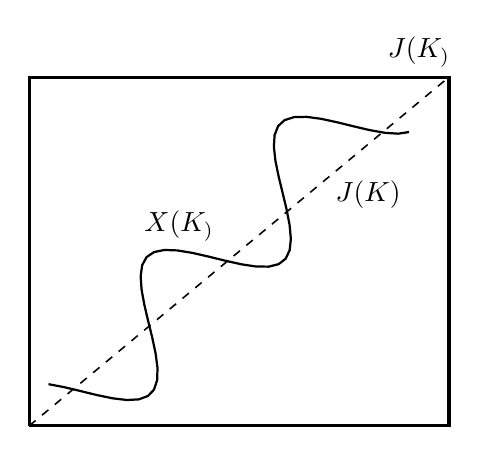
\begin{tikzpicture}
	\begin{axis}[
	hide axis,
	xmin=-3, xmax=6,
	ymin= -2, ymax= 7
	]
	\draw[line width=0.04cm] (-2,-1) -- (5,-1) -- (5,6) -- (-2,6) -- (-2,-1);
	\draw[line width= 0.02cm,dashed] (-2,-1) -- (5,6);
	\addplot[domain=-0.1*pi:2.2*pi, samples=50, black,thick,rotate=45] ({\x+0.5},{-sin(2*\x r)-3});
	\node at (0.5,3) {$X(K_\p)$};
	\node at (4.5,6.5) {$J(K_\p)$};
	\node at (3.65,3.65) {$J(K)$};
	\end{axis}
	\end{tikzpicture}
	\]
where $J(K_\p)$ is the completion of $K$ at $\p$ (a $p$-adic Lie group), the dotted line is the Mordell-Weil group $J(K)$ (a finitely generated abelian group, so a point and all its multiples, which can be dense), and $X(K_\p)$ is the set of local points on the curve (an analytic sub-manifold). The $K$-points of $X$ must lie on both $X(K_\p)$ and $J(K)$. To make this precise, we need an embedding (Abel-Jacobi map). Choose (assuming there is a $K$-rational point at all) $x \in X(K)$ to obtain an Abel-Jacobi map $X \hookrightarrow J$. 
	\[
	\begin{tikzcd}
	X(K) \arrow{r} \arrow{d} &  X(K_\p) \arrow{d} \\
	J(K) \arrow{r} & J(K_\p)
	\end{tikzcd}
	\]
Then the rational points map to rational points, with everything happening in the ambient Lie group $J(K_\p)$. Then we see that the rational points must be in the intersection of the local points $X(K_\p)$ and the Mordell-Weil group $J(K)$. This is the idea. We try to compute this intersection, hoping that the intersection is just the $K$-rational points with nothing `extra'. However in practice, this is difficult. Even writing down equations for $J(K)$ as a projective variety is `bad' enough---nevertheless trying to write down and explicitly work with its group law. So instead, we use the formal logarithm map obtained by integrating 1-forms $p$-adically. 
	\[
	\begin{tikzcd}
	X(K) \arrow{r} \arrow{d} &  X(K_\p) \arrow{d} \\
	J(K) \arrow{r} & J(K_\p) \arrow{r}{\log} & \lie J_{K_\p} \simeq K_\p^g
	\end{tikzcd}
	\]
where $J_{K_\p}$ is the base-change of $J(K)$ to the local field $K_\p$, i.e. an abelian variety defined over $K_\p$. Under this map, we transform the group law into addition in a vector space, which is much simpler to work with. So rather than trying to find the intersection of $X(K_\p)$ and $J(K)$ in $J(K_\p)$, we push everything `foward' and try to compute them in the vector space $K_\p^g$. [Notice the torsion subgroup `dies' because there is clearly no torsion in $K_\p^g$.]


Let's say a bit more about the log map. The log map is `close' to being an isomorphism. The kernel of the log map is finite (in fact, it is the torsion subgroup of $J(K_\p)$) and is a local diffeomorphism. Then the image of the log map will be open and compact ($J$ is a compact) subgroup of the $p$-adic vector space $K_\p^g$. [It is not necessarily an $\O_\p$-module, but it is a $\Z_\p$-module of full rank.] Therefore, the image of log is an open compact subgroup of the Lie group $\lie J_{K_\p}$. Moreover, the image of $J(K) \to K_\p^g$ is generated by $r$ elements, namely the generators of $J(K)$. Then the dimension of the $K_\p$-span of the image of the map $J(K) \to K_\p^g$ is at most $r$.


If $r< g$, there exists a nonzero linear functional $\lambda: \lie J_{K_\p} \to K_\p$ vanishing on $\im J(K)$, and $\lambda$ pulls back to a nonzero locally analytic function on $X(K_\p)$ vanishing on $X(K)$. Because on each residue disk $\lambda$ is a nonzero power series in a one-dimensional space, it has at most finitely many zeros on each closed disk (in this compact space). Therefore, $X(K)$ itself is finite. But of course, this all requires what might be called Chabauty's condition: $r<g$. If this condition fails, then the dotted points in our diagram could be dense, which would make it extremely difficult to find where they intersect the curve. 


Obviously, the difficulty in all of this is working with the Jacobian, which can be unwieldy. How do we limit the role of the Jacobian in this method? This idea was Kim's generalization. But before discussing that, let's see how we can restate this method while avoiding the use of Jacobians---the first step Kim had to take in his generalization. We begin with the same diagram as before, but now we $p$-adically complete the groups $J(K)$ and $J(K_\p)$, and invert $p$ in each. 
	\[
	\begin{tikzcd}
	X(K) \arrow{d} \arrow{r} & X(K_\p) \arrow{d} \\
	J(K) \arrow{r} \arrow{d} & J(K_\p) \arrow{r}{\log} \arrow{d} & \lie J_{K_\p} \\
	\widehat{J(K)}[\frac{1}{p}] & \widehat{J(K_\p)}[\frac{1}{p}] 
	\end{tikzcd}
	\]
Before continuing, we should remind the reader of $p$-adic completion. Given an abelian group $M$, we want to turn $M$ into a $\Z_p$-module. Define the $p$-adic completion to be $\hat{M}:= \plim M/p^nM$, which is a $\Z_p$-module. But of course, this is not a field. So we change this from $\Z_p$ to $\Q_p$ by localizing, i.e. inverting $p$. This is $\hat{M}[\frac{1}{p}] \simeq \hat{M} \otimes_{\Z_p} \Q_p$, which is a $\Q_p$ vector space. Now completion and localizing are functors, so we obtain a map $\widehat{J(K)}[\frac{1}{p}] \to \widehat{J(K_\p)}[\frac{1}{p}]$. From the discussion above, we knew that $\log$ was a local diffeomorphism. The only thing `getting in the way' of it being an isomorphism was torsion. But $\widehat{J(K_\p)}[\frac{1}{p}]$ is a $\Q_p$-vector space---there's no torsion left! This gives us the following diagram
	\[
	\begin{tikzcd}
	X(K) \arrow{d} \arrow{r} & X(K_\p) \arrow{d} \\
	J(K) \arrow{r} \arrow{d} & J(K_\p) \arrow{r}{\log} \arrow{d} & \lie J_{K_\p} \\
	\widehat{J(K)}[\frac{1}{p}] \arrow{r} & \widehat{J(K_\p)}[\frac{1}{p}] \arrow{ur}{\rotatebox{45}{$\sim$}} 
	\end{tikzcd}
	\]
 

The next step is to re-express everything in terms of \etale homology. In 2-descent for elliptic curves, we look at the map $E(K)/2E(K) \to H^1(K,E[2])$, i.e. the Kummer map. Everything we have is built from quotients that behave like this, e.g. $J(K)/pJ(K)$. So there should be a analogous descent into some Galois cohomology. This something is the cohomology of the Galois group of $K$ acting on some kind of Tate module, which we will write $H^1(K,V)$, and its local version $H^1(K_\p,V)$. But what is $V$? We can think of $V$ as some kind of \etale homology.\footnote{See David Corwin's notes \href{https://math.berkeley.edu/~dcorwin/files/ChabautytoKim.pdf}{From Chabauty's method to Kim's non-abelian Chabauty method}} 


As a motivation, if $X$ is a curve over $\C$ and $J$ is its Jacobian, then analytically as a complex manifold, $J(\C) \simeq \C^g/ \Lambda$, where $\Lambda$ is a rank $2g$ lattice. But $\Lambda$ is also the fundamental group of the space, easily seen from the fact that the universal cover is $\C^g$. Then we can view $\Lambda$ as the homology $\Lambda= H_1(J(\C),\Z)$. Of course, viewing $J(\C)$ as $\C^g/\Lambda$ is far simpler because the group law has been turned into `traditional' addition. Viewing $J(\C)$ as $\C^g/\Lambda$, it is easy to see that 
	\[
	J[p] \simeq \frac{1}{p} \Lambda/\Lambda \ma{\stackrel{p}{\sim}} \Lambda/p\Lambda= H_1(J(\C), \Z/p\Z)= H_1(X(\C),\Z/p\Z) 
	\]
where we have used the homology groups, $H_1$, for curves and their Jacobians are the same. But now there is no $J$ involved! So we can talk about the $p$-torsion of the Jacobian without actually involving $J$. This can be done similarly for the $p^n$-torsion, and so on. 


We want to create an analog of this for a curve that is not over the complex numbers. But if we are not using $\C$, we are going to have to switch to \Etale (co)homology. For $X$ over $K$, $J[p] \simeq H_1^\et(X_{\ov{K}}, \Z/p\Z):= \Z/p\Z$-dual of $H^1_\et(X_{\ov{K}}, \Z/p\Z)$. [Note, one should only take \etale (co)homology of a geometric object, so be sure to base change to an algebraic closure first.] Similarly, $J[p^n] \simeq H_1^\et(X_{\ov{K}}, \Z/p^n\Z)$. Now taking inverse limits, we obtain the $\Z_p$ Tate module $T:= \plim J[p^n] \simeq H_1^\et(X_{\ov{K}}, \Z_p)$. Again to avoid rings that are not fields, tensoring with $\Q_p$, we obtain the $\Q_p$ Tate module $V:= T[\frac{1}{p}]= T \otimes_{\Z_p} \Q_p \simeq H_1^\et(X_{\ov{K}}, \Q_p)$ obtained by inverting $p$, which is a $\Q_p$-vector space of dimension $2g$. There is always a way of moving from a vector space to an algebraic group whose points are the vector space. Because it will later be useful to think of $V$ in this way, write $\cV(\Q_p)$ for a group variety $\cV \simeq \G_a^{2g}$, the group variety over $\Q_p$. As a variety, $\cV$ is $\A^{2g}$ with an additive group law (coordinate-wise addition). The group $G_K:= \Gal(\ov{K}/K)$ acts continuously on all of these, e.g. $G_K \to \Aut \cV \simeq \GL_n(\Q_p)$, as a group variety. 

